% This is "sig-alternate.tex" V2.0 May 2012
% This file should be compiled with V2.5 of "sig-alternate.cls" May 2012
%
% This example file demonstrates the use of the 'sig-alternate.cls'
% V2.5 LaTeX2e document class file. It is for those submitting
% articles to ACM Conference Proceedings WHO DO NOT WISH TO
% STRICTLY ADHERE TO THE SIGS (PUBS-BOARD-ENDORSED) STYLE.
% The 'sig-alternate.cls' file will produce a similar-looking,
% albeit, 'tighter' paper resulting in, invariably, fewer pages.
%
% ----------------------------------------------------------------------------------------------------------------
% This .tex file (and associated .cls V2.5) produces:
%       1) The Permission Statement
%       2) The Conference (location) Info information
%       3) The Copyright Line with ACM data
%       4) NO page numbers
%
% as against the acm_proc_article-sp.cls file which
% DOES NOT produce 1) thru' 3) above.
%
% Using 'sig-alternate.cls' you have control, however, from within
% the source .tex file, over both the CopyrightYear
% (defaulted to 200X) and the ACM Copyright Data
% (defaulted to X-XXXXX-XX-X/XX/XX).
% e.g.
% \CopyrightYear{2007} will cause 2007 to appear in the copyright line.
% \crdata{0-12345-67-8/90/12} will cause 0-12345-67-8/90/12 to appear in the copyright line.
%
% ---------------------------------------------------------------------------------------------------------------
% This .tex source is an example which *does* use
% the .bib file (from which the .bbl file % is produced).
% REMEMBER HOWEVER: After having produced the .bbl file,
% and prior to final submission, you *NEED* to 'insert'
% your .bbl file into your source .tex file so as to provide
% ONE 'self-contained' source file.
%
% ================= IF YOU HAVE QUESTIONS =======================
% Questions regarding the SIGS styles, SIGS policies and
% procedures, Conferences etc. should be sent to
% Adrienne Griscti (griscti@acm.org)
%
% Technical questions _only_ to
% Gerald Murray (murray@hq.acm.org)
% ===============================================================
%
% For tracking purposes - this is V2.0 - May 2012

\documentclass{sig-alternate}
\usepackage{url}

\begin{document}
\conferenceinfo{GECCO'13,} {July 6-10, 2013, Amsterdam, The Netherlands.}
\CopyrightYear{2013}
\crdata{TBA}
\clubpenalty=10000
\widowpenalty = 10000


%
% --- Author Metadata here ---
%\conferenceinfo{WOODSTOCK}{'97 El Paso, Texas USA}
%\CopyrightYear{2007} % Allows default copyright year (20XX) to be over-ridden - IF NEED BE.
%\crdata{0-12345-67-8/90/01}  % Allows default copyright data (0-89791-88-6/97/05) to be over-ridden - IF NEED BE.
% --- End of Author Metadata ---

\title{EvoSpace-Interactive: A framework for Interactive Evolutionary Algorithms}
%\titlenote{A full version of this paper is available as
%\textit{Author's Guide to Preparing ACM SIG Proceedings Using
%\LaTeX$2_\epsilon$\ and BibTeX} at
%\texttt{www.acm.org/eaddress.htm}}}
%
% You need the command \numberofauthors to handle the 'placement
% and alignment' of the authors beneath the title.
%
% For aesthetic reasons, we recommend 'three authors at a time'
% i.e. three 'name/affiliation blocks' be placed beneath the title.
%
% NOTE: You are NOT restricted in how many 'rows' of
% "name/affiliations" may appear. We just ask that you restrict
% the number of 'columns' to three.
%
% Because of the available 'opening page real-estate'
% we ask you to refrain from putting more than six authors
% (two rows with three columns) beneath the article title.
% More than six makes the first-page appear very cluttered indeed.
%
% Use the \alignauthor commands to handle the names
% and affiliations for an 'aesthetic maximum' of six authors.
% Add names, affiliations, addresses for
% the seventh etc. author(s) as the argument for the
% \additionalauthors command.
% These 'additional authors' will be output/set for you
% without further effort on your part as the last section in
% the body of your article BEFORE References or any Appendices.

\numberofauthors{5} %  in this sample file, there are a *total*
% of EIGHT authors. SIX appear on the 'first-page' (for formatting
% reasons) and the remaining two appear in the \additionalauthors section.
%
\author{
% You can go ahead and credit any number of authors here,
% e.g. one 'row of three' or two rows (consisting of one row of three
% and a second row of one, two or three).
%
% The command \alignauthor (no curly braces needed) should
% precede each author name, affiliation/snail-mail address an
% e-mail address. Additionally, tag each line of
% affiliation/address with \affaddr, and tag the
% e-mail address with \email.
%
% 1st. author
\alignauthor
author's names removed\\
%       \affaddr{Institute for Clarity in Documentation}\\
%       \affaddr{1932 Wallamaloo Lane}\\
%       \affaddr{Wallamaloo, New Zealand}\\
%       \email{trovato@corporation.com}
% 2nd. author
%\alignauthor
%G.K.M. Tobin\titlenote{The secretary disavows
%any knowledge of this author's actions.}\\
%       \affaddr{Institute for Clarity in Documentation}\\
%       \affaddr{P.O. Box 1212}\\
%       \affaddr{Dublin, Ohio 43017-6221}\\
%       \email{webmaster marysville-ohio.com}
% 3rd. author
%\alignauthor Lars Th{\o}rv{\"a}ld\titlenote{This author is the
%one who did all the really hard work.}\\
%       \affaddr{The Th{\o}rv{\"a}ld Group}\\
%       \affaddr{1 Th{\o}rv{\"a}ld Circle}\\
%       \affaddr{Hekla, Iceland}\\
%       \email{larst ffiliation.org}
}
% There's nothing stopping you putting the seventh, eighth, etc.
% author on the opening page (as the 'third row') but we ask,
% for aesthetic reasons that you place these 'additional authors'
% in the \additional authors block, viz.
%\additionalauthors{Additional authors: John Smith (The Th{\o}rv{\"a}ld Group,
%email: {\texttt{jsmith@affiliation.org}}) and Julius P.~Kumquat
%(The Kumquat Consortium, email: {\texttt{jpkumquat@consortium.net}}).}
%\date{30 July 1999}
% Just remember to make sure that the TOTAL number of authors
% is the number that will appear on the first page PLUS the
% number that will appear in the \additionalauthors section.

\maketitle
\begin{abstract}
	

This work presents EvoSpace-Interactive, an open source framework for
the development of collaborative-interactive evolutionary algorithms
for art and design. The main components of the framework are i)
Evospace, a population store for the development of % por qué no
                                % EvoStore? - JJ
cloud-based evolutionary algorithms, implemented using Redis key-value
server and ii) Interactive, % por qué no EvoAgent? La división entre
                            % los dos nombres no me parece muy
                            % descriptiva- JJ
an application based on the Django framework that allows 
 end-users to collaborate in a social network sharing, collecting,
 rating and ultimately evolving individuals. Individuals are presented
 as multimedia elements (images, animations, sound clips) using the
 Processing programming language. Details of the design are presented
 and two example applications that illustrate the potential of
 the tool are shown. % No me gusta shown. Explained? Presented?
                     % Described? - JJ
\end{abstract}

% A category with the (minimum) three required fields
\category{H.4}{Information Systems Applications}{Miscellaneous}
%A category including the fourth, optional field follows...
\category{D.2.8}{Software Engineering}{Metrics}[complexity measures, performance measures]

%\terms{Theory}

\keywords{ Interactive evolutionary computation, Interactive Systems, Cloud-based platforms}

\section{Introduction}
\section{Related Work}


\section{Architecture}
The goal of this work is to develop an open source framework for Web and Cloud-based C-IEA systems,
using current web standards and libraries for mobile devices. 
Developers of C-IEA applications are liberated from the need to design and program a platform for distributed user collaboration.
Only three components of the framework  must to be defined for each
application (marked with double lines in Figure \ref{fig:arch}), namely: an \emph{individual} representation; a \emph{processing script} that renders each individual; and a \emph{worker} script that encodes the evolutionary operators will need to be defined according to the representation and problem domain.
However, in future versions of the framework much of this work could be predefined, but also left open for advanced users to change as they require.
What the framework offers for free is: a central repository for the population implemented as an EvoSpace service; a Web Application script implemented using Django, a mature full stack Web Framework with a BSD license developed in Python.


The main components of the EvoSpace-Interactive are shown in Figure~\ref{fig:arch}. The Interactive part is a Django \cite{} web-based application, together with a client-side component implemented using JQuery and processingjs Javascript libraries. This application shows users a number of multimedia objects rendered in HTML5 Canvas elements. These multimedia objects are the phenotypes of individuals drawn from the Evospace population store. Evospace is responsible for storing and retrieving the data of each individual. An Evolution Worker is responsible for generating new individuals from a sample taken from EvoSpace. The evolution process is decoupled from the interactive application; thous giving IEC designers the opportunity to define their own variations of the algorithm. In the following sections each component is described in detail, staring with the population store Evospace, and then the Interactive and Collaborative components.     

\begin{figure*}[!t]
    \centering
        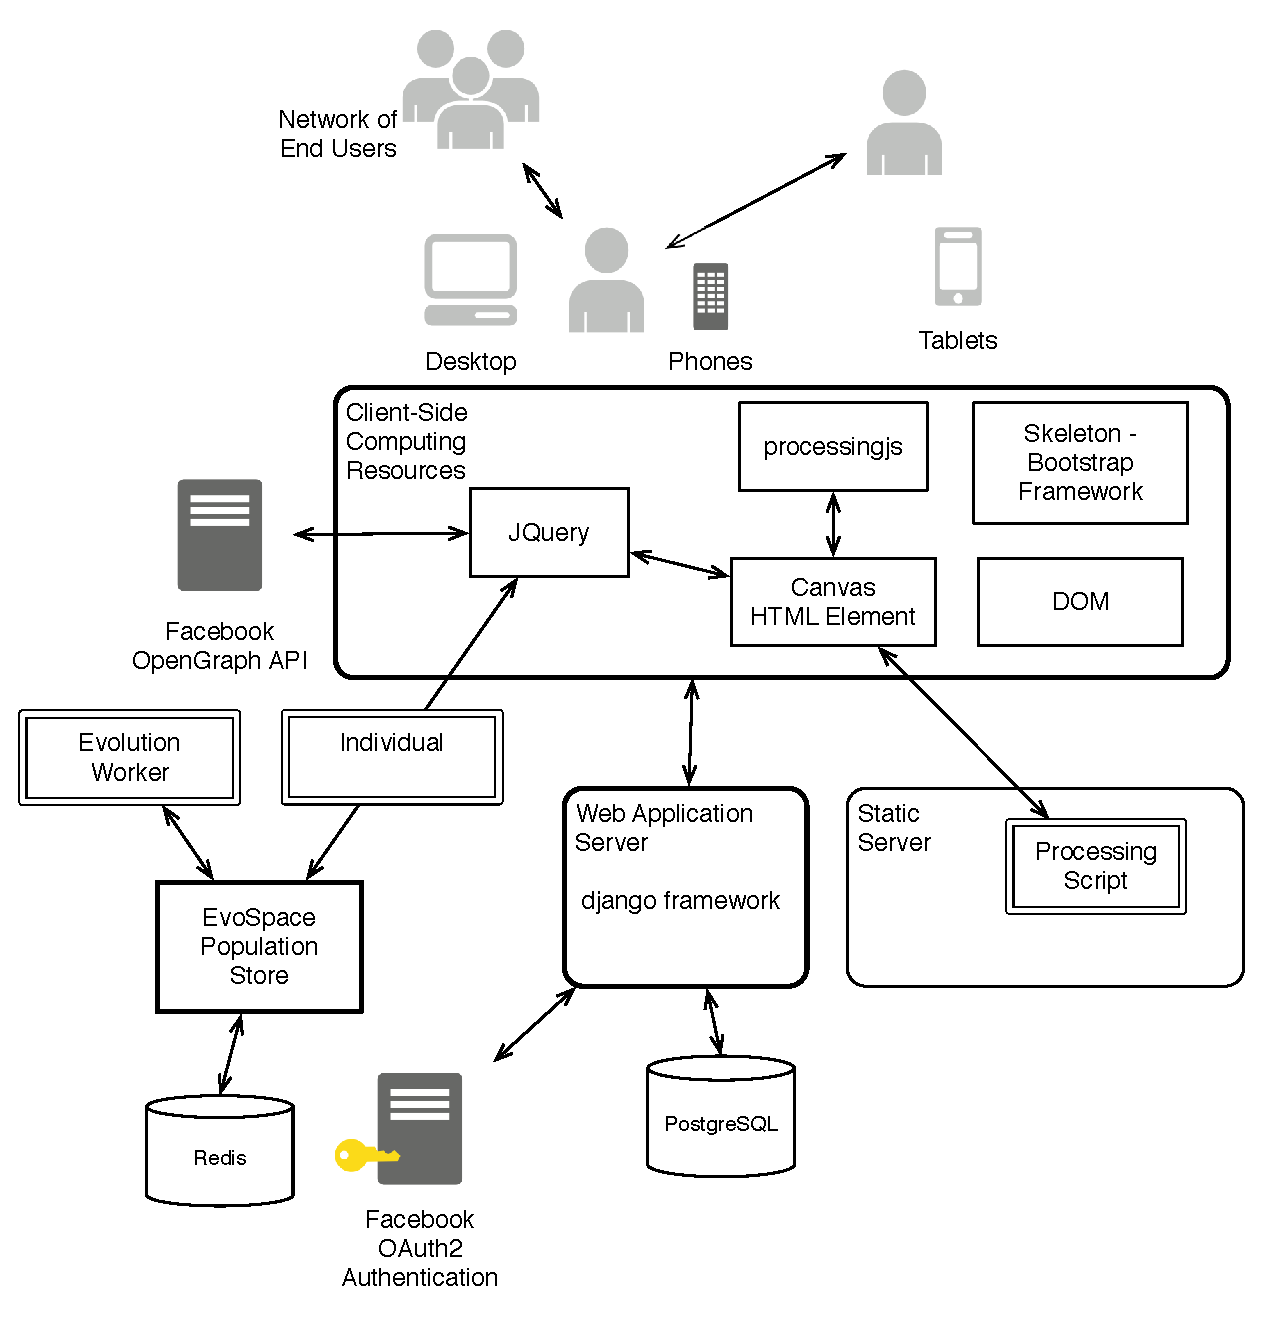
\includegraphics[width=4.5in]{Architecture.eps}
    \caption{Main components of EvoSpace-Interactive.}
    \label{fig:arch}
\end{figure*}


\section{EvoSpace} % debería ser EvoSpace-i - JJ
The EvoSpace model is presented in detail in \cite{EvoSpace}, only
brief description of the functionality related to this work is given
next.  EvoSpace is inspired on the Linda language by Gelernter and
Carriero \cite{linda}; Linda is a model of coordination and
communication among several parallel processes operating upon objects
stored in and retrieved from a shared, virtual, associative memory
called {\em tuplespace}. In a tuplespace, tuples are read and removed by processes; once a tuple is taken, no other process can read it until it is written back. EvoSpace consists of two main components (see figure~\ref{fig:evo}):\begin{itemize}
\item the EvoSpace container
that stores the evolving population and
\item remote clients called
EvoWorkers, % ajústate a la terminología del abstract, "Evospace" +
            % "interactive" o "EvoStorage + EvoWorkers" - JJ
which execute the actual evolutionary process, while EvoSpace acts
only as a population repository. 
\end{itemize}

In a basic configuration, EvoWorkers take a random sample of the
population, and use it as the initial population for a local EA
executed on the client machine. When taken by an EvoWorker,
individuals  remain in a phantom state until their sample is
returned. If an EvoWorker does not returns a sample in a certain
amount of time, for instance because of a lost connection; individuals
are re-spawned (re-inserted) by the ReInsertionManager. Similar to
video games in which characters once killed are re-spawned after a
certain time. This can also happen when the EvoSpace container starves
or the population size is below some threshold. Figure~\ref{fig:evo}
illustrates the main components and dataflow within EvoSpace. % Ni lo
                                % explicas aquí ni en el pie de
                                % figura. Deberías explicarlo un poco
                                % más - JJ

For this version of EvoSpace-Interactive, a new type of Worker is needed: Human users. Users are responsible for subjectively evaluating individuals, the process is depicted in Figure~\ref{fig:evoInteractive}: (i) first a random sample of six individuals are taken from EvoSpace, (ii) the chromosome of each individual parameterizes a Processing script, that renders to the user, (iii) users select those individuals they like, this is stored in each individual's data, (iv) finally the sample is returned to EvoSpace. The fitness assigned to each individual can depend on the ratings given by a certain number of users. In this case the EvoWorker process is replaced  by an \texttt{Evolve} method, that is executed after a certain number of samples have been returned. 
Unlike the normal operation of EvoSpace, when a User takes a sample of users, these are returned with their identity unchanged, other than the rating added by the current user. The internal representation of individuals is presented next.

\paragraph{Individuals.} % Por qué paragraph y no subsection? Además,
                         % tiene dos puntos - JJ
As stated above, the objects stored in EvoSpace are individuals in an EA.
Explicitly, individuals are stored as \emph{dictionaries}, an abstract data type that represents a collection of unique keys and values with a one to one association. In this case, keys represent specific properties of each object and the values can be of different types, such as
numbers, strings, lists, tuples or other dictionaries.
In the current implementation, individuals are described by the following basic fields.
An \textbf{id} string that represents a unique identifier for each object.
A \textbf{chromosome} string, which depends on the EA and the representation used.
The \textbf{fitness} dictionary for each individual; In EvoSpace-Interactive it stores pairs of user's ids and timestamp values, which represent that a user has rated the individual with a like. Currently a user can rate more than one time each individual.
The \textbf{views} The number of times the individual has been presented to a user. If a user has seen an individual and  did not assigned it a like, this can be used as a probable not-like rating.
A \textbf{parents} dictionary with identifiers of the individual(s) from which it was produced.
Finally, a \textbf{GeneticOperator}  string that specifies the operator that produced it.   


Individuals are stored in-memory, using the Redis key-value database. Redis was chosen over a SQL-based management system, or other non-SQL alternatives, because it provides a hash based implementation of sets and queues which are natural data structures for the EvoSpace model. For example, selecting a random key from a set has a complexity of O(1). The logic of EvoSpace is implemented as a python module exposed by the same Django framework used by the web-based application. The EvoSpace web service interacts is called directly by a JQuery script running in the client-side. This is done by a JQuery ajax request, and using the  JSON-RPC protocol.  The EvoSpace module is available with a Simplified BSD License from \url{https://github.com/evoWeb/EvoSpace}.  The components required for the interaction between individuals and users are presented next.

\begin{figure}[!t]
    \centering
        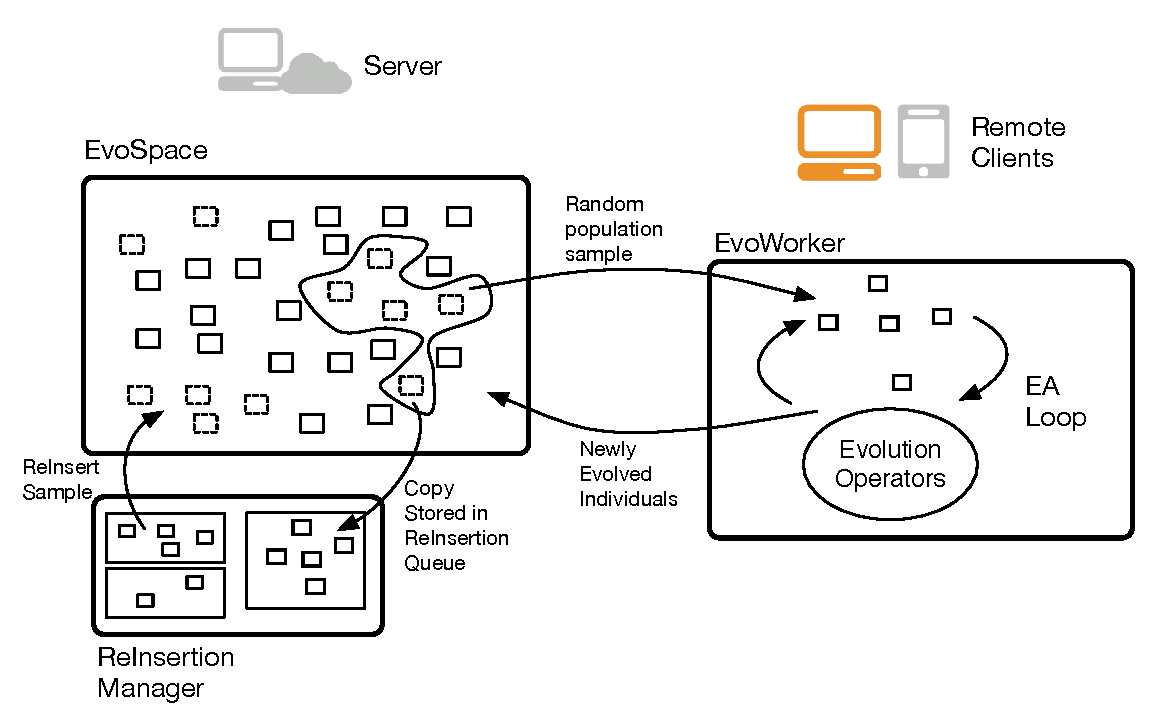
\includegraphics[width=3.5in]{evospaceExample.eps}
    \caption{Main components and dataflow within EvoSpace.}
    \label{fig:evo}
\end{figure}



\begin{figure}[!t]
    \centering
        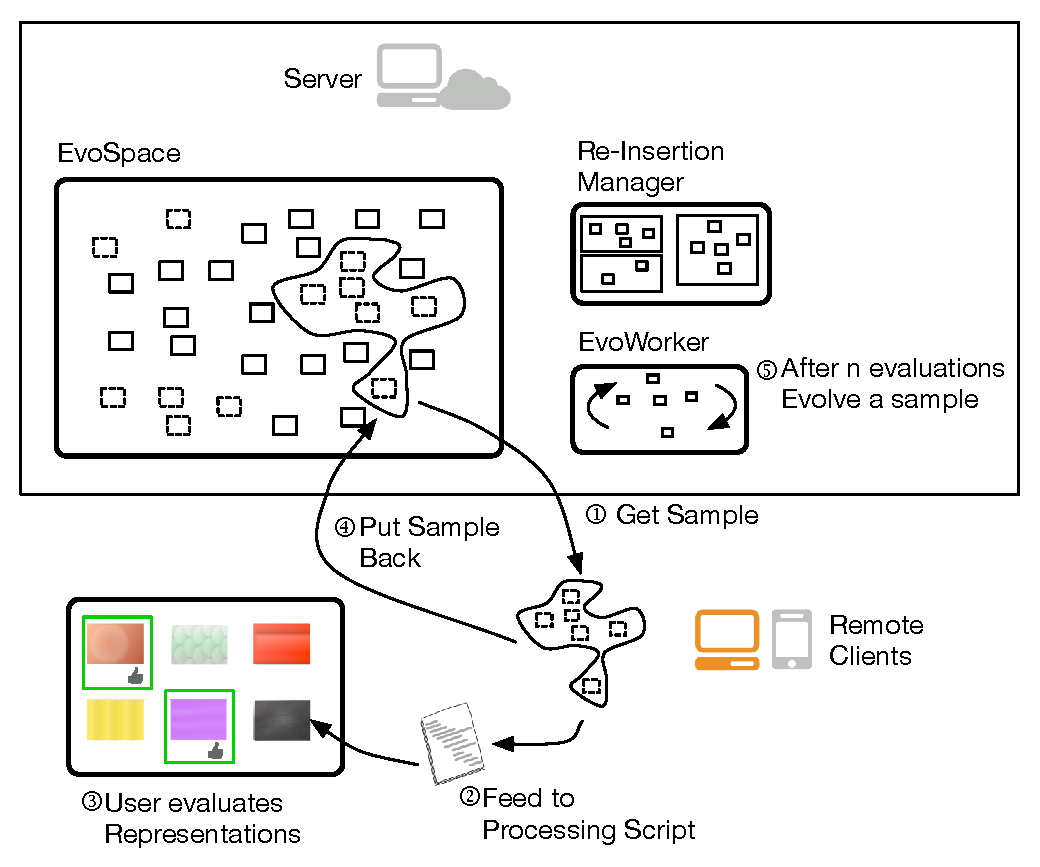
\includegraphics[width=3.5in]{evospaceInteractive.eps}
    \caption{}
    \label{fig:evoInteractive}
\end{figure}


\section{Interactive Evolution}
In this section, the components needed to enable the interaction between users and individuals are presented. The first subsection the rendering and representation of individuals is discussed and next how fitness is assigned.

\subsection{Processing Scripts}
Processing is a programming language and development environment initially created to serve as a software sketchbook and as a tool to teach fundamentals
of computer programming within a visual context.
Currently is used by artists, designers, architects, and researchers for visualization applications, games and interactive animations projects \cite{Reas:2007wp}.
Processing is a subset of Java directed to novice programmers and generative artists \cite{Pearson:2011ti}, which are the intended users of the EvoSpace-Interactive framework.
As a complement there is a javascript library \emph{processingjs} that allows Processing scripts to be run by any HTML5 compatible browser.
Processing scripts are responsible of rendering individuals which can involve animations, sound or even interactive artifacts.
Before calling the \texttt{draw()} method of the processing script a local array of parameters are replaced with those of each individual's chromosome.
Each individual's script has its own Canvas entity; defined by the HTML5 standard, as an element that provides scripts with a resolution-dependent bitmap canvas which can be used for rendering graphics on the fly.
Although the combination of an HTML5 Canvas element and a Processing script is supported by default, other combinations could be used.
For instance, images, embedded audio, or other libraries capable of drawing in the Canvas.
Also, a fallback implementation must be considered for applications intended for non-HTML5 capable browsers.

To create a new C-IEC application, the  rendering script must be defined, and its parameters encoded as a chromosome.    


\subsection{Fitness}
As stated before, the assignment of the fitness for each individual takes into account the evaluation given by several users. Initially in EvoSpace-Interactive users can only give positive evaluations explicitly when they select an individual, giving it a rating of \emph{Like}.
When a user evaluates a sample of individuals, some (or all) of them will not receive a like, in each case the \texttt{views} property will be incremented by 1. For instance, if an individual has a high number of views with with only two likes, he considered to be  worse than an individual with two views and two likes. The ratio $Likes/Views$ is more informative, but it does not distinguish between an individual with many views and another with only
one view if they both have zero likes; also views must be >=1 to avoid dividing by zero. Fitness, therefore, it is proposed to be given by $(Likes+1)/(Views+1)$. As a future work more options can be defined, for instance taking into account the number of ``shares'' or the times an individual has been stored in a collection. 

\subsection{Breeding Process}

Once individuals have been evaluated by a minimum number of users, these can participate in the breeding process. As the genetic operators of the evolution process, will depend of the particular application; this algorithm must be implemented in python. Python libraries as DEAP or PyEvolve can be used for this purpose. Both examples presented in this work were implemented using only the NumPy library for array operations. As this process is executed in the server, the communication with EvoSpace-Redis is directly through a library. Only clients connect to the Web Service. There are a few additional parameters that are used for the \texttt{Evolve()} method: \texttt{EVOLUTION-INTERVAL} indicates the number of that must returned to trigger an \texttt{Evolve()} call; the  \texttt{SAMPLE-SIZE} parameter indicates how many individuals are taken from EvoSpace to participate in the Evolution, \texttt{MINIMUM-VIEWS} is the minimum views needed for each individual to participate in the breeding process.

\section{Collaboration}
Using their Facebook account, users can collaborate with their Facebook friends, sharing those individuals they like, or taking individual from the collections of friends, as an introduction to this section de general user experience is described next.

\subsection{User Interface.}
Users interact with the web interface depicted in Figure \ref{fig:web}, which is composed of five elements.
First, at the top left corner user login and authentication.
Users can login with their Facebook account or participate as anonymous users.
Second, if a user chooses to login a list of Facebook friends that have also linked their account with the C-IEA application is presented on the left, to encourage users to interact with the system. The third element is a central \emph{ Wall } area, where a population sample of $n$ individuals is shown to the user.
These are $n$ random individuals taken from the EvoSpace server.
Here, the user can interact with the system in two ways.
He can click on the individuals he prefers, a clicked image is highlighted and this counts as a ``like'' for the individual.
Additionally, a user can choose to add an image to one of their \emph{Collections}.
A collection is a special directory to store individuals a user prefers and wishes to save. After the user finishes interacting with the current crop of individuals on the Wall, he can choose to retrieve a new sample from EvoSpace.
This is done with the fourth element of the interface, located at the top of the screen, the \emph{GetMore} button.
The button returns the current group of individuals to EvoSpace, and brings back a new one.
Each time a user performs a \emph{GetMore} click, it increments the number of samples returned, and this could  trigger a server-side \emph{Evolve()} method. The fifth element of the interface is shown at the bottom left corner, the \emph{Collections} section.
The user can create several collections, to group and organize his favorite artifacts.
Moreover, a user can browse the content of each collection and from there share images through the social network.
When a user browses over an individual a detail pane shows how many users have liked the individual.
The pane also includes a link to the individual's details, the parents, genetic operators that created it, and genealogy information.


\begin{figure}[!t]
    \centering
        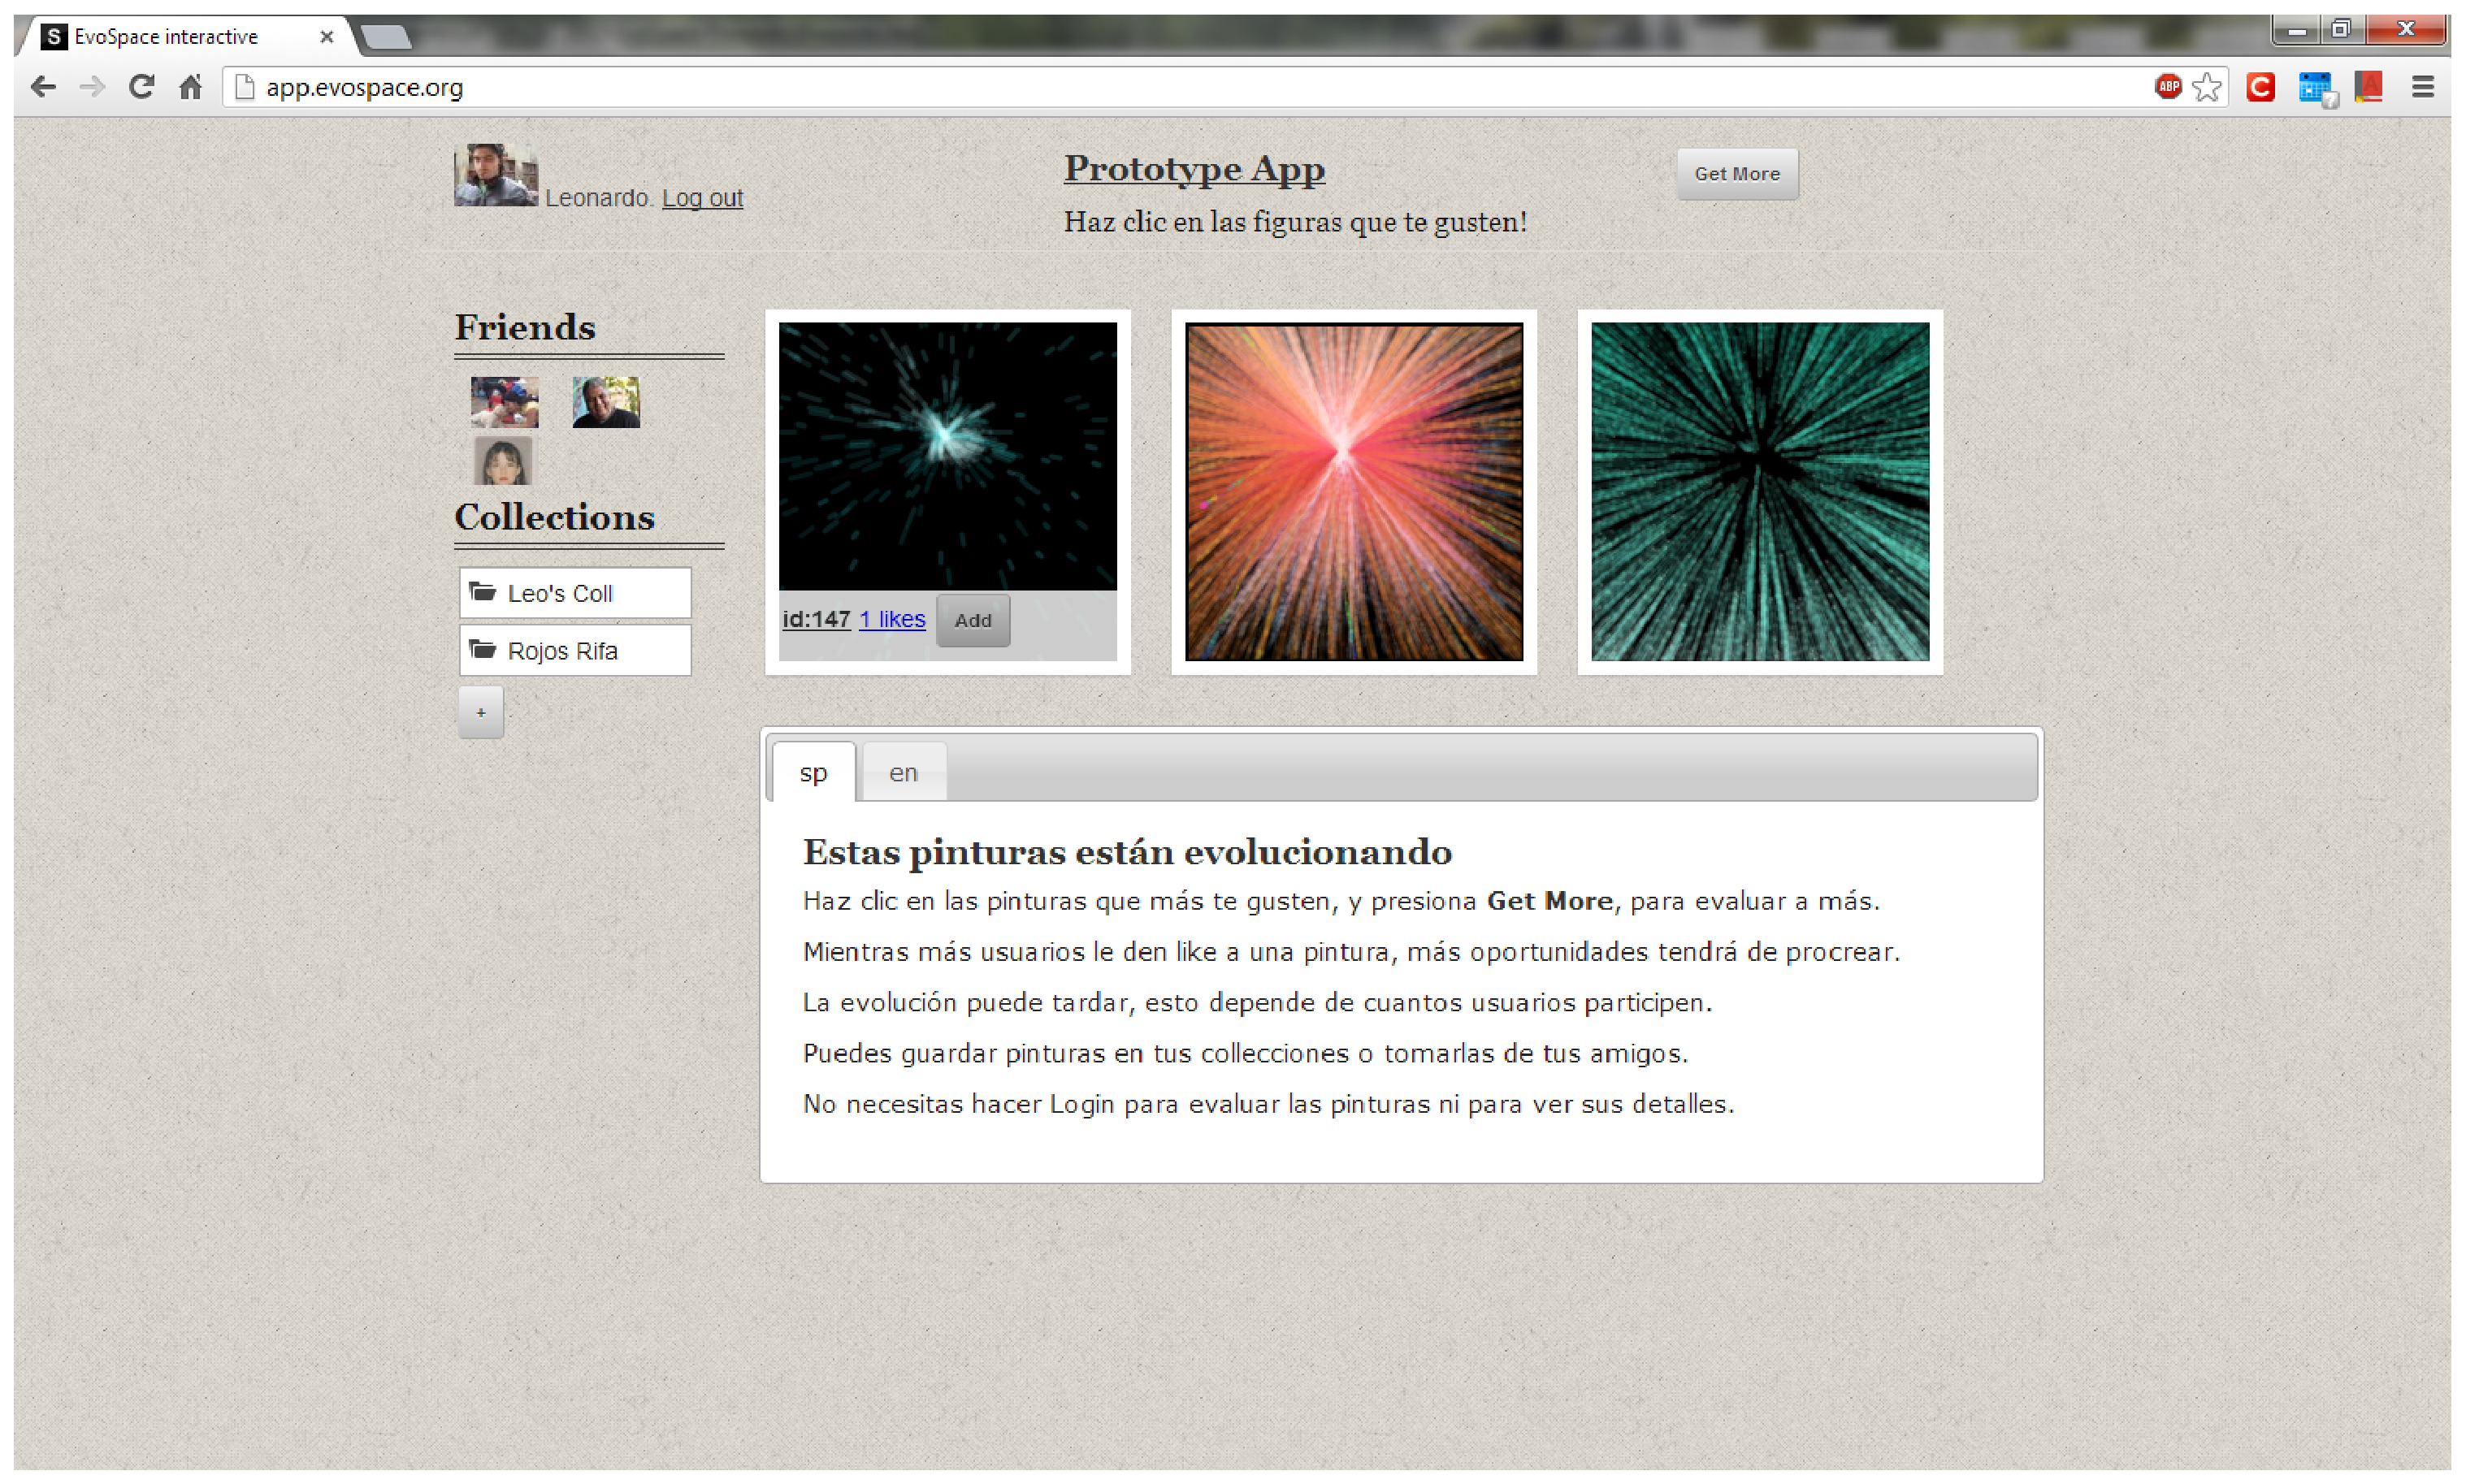
\includegraphics[width=3.5in]{EvoApp.eps}
    \caption{}
    \label{fig:web}
\end{figure}

\subsection{Facebook API and OAuth2.0}
Applications developed with the EvoSpace-Interactive framework must be defined as Facebook Web Applications. Other social networks are going to be enabled in further versions of the framework; but initially Facebook was selected as a Social Network platform for the following reasons:
\begin{itemize}
	\item Popularity. Facebook is currently the social network with more active users, with more than 1 billion. 

	\item Applications. Facebook applications are also common, popular applications like Youtube, Pinterest, Netflix, XBOX Live and Spotify allow users to share their activities.	
\end{itemize}
In order to enable the application's collaborative functionality, end-users must be authenticated with their Facebook account. This is done using the OAuth2.0 protocol \cite{hammer2011oauth}. The OAuth 2.0 login flow generates an access token, which you can use to make API calls on behalf of a user. As part of this flow, users also give certain permissions to the application, so it can access their private data. Currently the framework uses the most basic permission, having access only to their public profile and list of friends. The public profile includes their profile picture, username, gender and locale. An important information is the list of friends, that includes which friends also have the application installed. 

\subsection{Django Framework Application}
The Django web development framework \cite{django}, is a set of Python libraries, that provide high-level abstractions of common Web development patterns. In Django a web application consists of different python scripts following a Model-View-Controller (MVC) design pattern. Using a separation of concerns design principle, the application logic is separated in mainly in four scripts:
\begin{itemize}
	\item The \texttt{models.py} script contains a class based description of the database schema. These classes are Object-Relational mappers with methods to create, retrieve, update, and delete records in your database using Python code instead of SQL.
	\item The \texttt{views.py} file contains the business logic for each web page defined as special  ``View'' functions. These functions receive as parameters and http request data, do operations on the model (database) , and return the data to feed HTML generator templates. 
	\item The \texttt{urls.py} file specifies which view is called for a given URL pattern.
    \item Various HTML template files that describes the design of the page.
    \item \texttt{settings.py} file where the configuration of the project is stored.
\end{itemize}

In Django, a project can be an aggregation of multiple reusable applications, each incorporating a particular functionality. Each application has its own model, and views. For EvoSpace-Interactive the database model is presented in Figure~\ref{datamodel}. There is a many to one relationship between facebook sessions and users, this is because sessions and access tokens can expire. The database is stored in a PostgreSQL database system. Individuals are not stored in this database, they are stored in a Redis server as JSON text. The model for individual is presented in Figure~\ref{redisModel}   

\begin{figure}[!t]
    \centering
        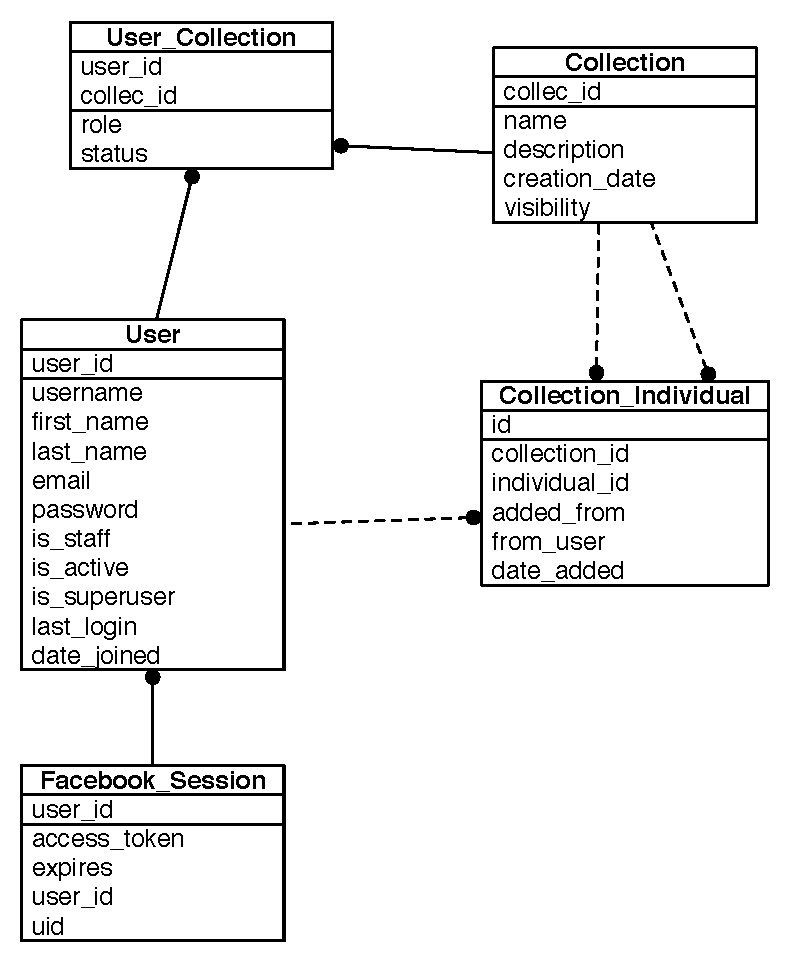
\includegraphics[width=3.5in]{datamodel.eps}
    \caption{Django data model for the Interactive application}
    \label{datamodel}
\end{figure}

\begin{figure}[!t]
    \centering
        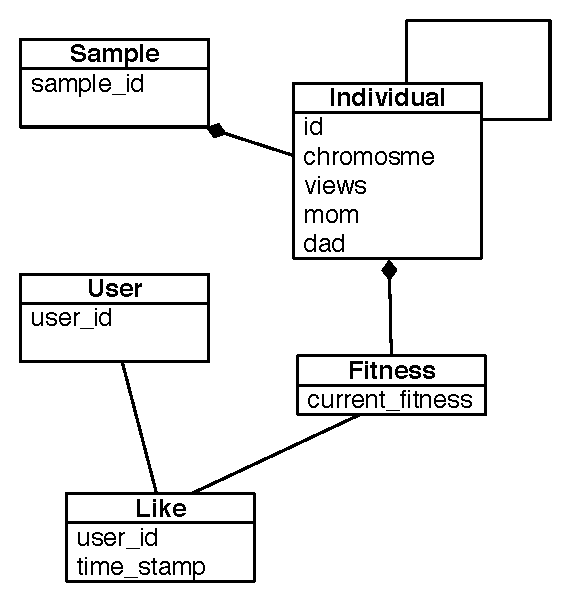
\includegraphics[width=3in]{redisModel.eps}
    \caption{Individual's JSON representation}
    \label{redisModel}
\end{figure}

The main view functions for the application are:

\begin{description}

\item[\texttt{evospace()}] This function receives JSON-RPC requests from JQuery code in the client. Main methods are \texttt{getSample() } and \texttt{putSample()}. 
\item[\texttt{home()}] This view is for the main page, if the user is authenticated the list of friends and profile data is retrieved.
\item [\texttt{individual\_view()}] This view function returns the details of Individuals.
\item [\texttt{facebook\_login()}] Initializes the OAuth 2.0 flow. The facebook\_get\_login is also related.
\item [\texttt{dashboard()}] Returns a JQuery dashboard page, for administration of EvoSpace.
\end{description}

\subsection{Client-Side}
Client-side scripting is used extensibly by the framework. As mentioned earlier, JQuery is used to implement the evaluation of individuals as shown earlier in Figure~\ref{fig:evoInteractive}, sending \texttt{getSample()} and \texttt{putSample()} requests.  Also the Javascript library processingjs is used to render each individual in its corresponding HTML5 Canvas element. Other controls such as Modal Windows, Lists, Buttons are also implemented using JQuery-UI library.
    
\subsection{Collections}
TO-DO
\section{Example Application}
As a proof of concept a C-EIA application was implemented with the EvoSpace-Interactive framework, this application is detailed in \cite{Musart}. The application is called \emph{Shapes}, and implements each EvoSpace-Interactive component as follows.

In \emph{Shapes}, individuals represent a two dimensional 11 by 6 array of equilateral triangles, these arrays are sometimes used in Op-Art style paintings.
Each triangle has a color drawn from a twelve color palette.
The array is represented by a 66 element chromosome vector $\mathbf{v}=(v_1,..v_{66})$, with $v_i \in \{ 1,2,..11 \}$.
The background of the painting is Light Gray, this can give the effect of a missing triangle when it has the same color.
A processing script is used to render a static version of the image.
The breeding process uses tournament selection of size 6 to select two individuals from EvoSpace,
and generates two offspring.
The offspring replace the worst individuals from both tournament groups.
Crossover operators are used with crossover rate of 1, these are vertical and horizontal one-point crossovers.
Several mutations are used with a mutation rate of 0.3, these are:
(1) single \emph{point mutation}; (2) vertical and horizontal \emph{mirrors} at a random point;
(3) \emph{shuffle} that gives a new permutation of the chromosome.

\section{Evaluation}
TO-DO
\section{Conclusions}
TO-DO

%\end{document}  % This is where a 'short' article might terminate

%ACKNOWLEDGMENTS are optional
\section{Acknowledgments}
This work is supported by projects 4616.12-P and 4617.12-P awarded by DEGEST-ProIFOPEP (Mexico), TIN2011-28627-C04-03 and -02 (ANYSELF), awarded by the Spanish Ministry of Science and Innovation, P08-TIC-03903 (EvOrq) awarded by the Andalusian Regional Government, project 83 (CANUBE) awarded by the CEI-BioTIC UGR
(\url{http://biotic.ugr.es}) and CONACYT (Mexico) Basic Science Research Project No. 178323 and DGEST (Mexico) Research Project No. TIJ-ING-2012-110.

%
% The following two commands are all you need in the
% initial runs of your .tex file to
% produce the bibliography for the citations in your paper.
\bibliographystyle{abbrv}
\bibliography{evospace-i}  % sigproc.bib is the name of the Bibliography in this case
% You must have a proper ".bib" file
%  and remember to run:
% latex bibtex latex latex
% to resolve all references
%
% ACM needs 'a single self-contained file'!
%
%APPENDICES are optional
%\balancecolumns



\end{document}
